\documentclass[12pt,letterpaper]{article}
\usepackage{graphicx,textcomp}
\usepackage{natbib}
\usepackage{setspace}
\usepackage{fullpage}
\usepackage{color}
\usepackage[reqno]{amsmath}
\usepackage{amsthm}
\usepackage{fancyvrb}
\usepackage{amssymb,enumerate}
\usepackage[all]{xy}
\usepackage{endnotes}
\usepackage{lscape}
\newtheorem{com}{Comment}
\usepackage{float}
\usepackage{hyperref}
\newtheorem{lem} {Lemma}
\newtheorem{prop}{Proposition}
\newtheorem{thm}{Theorem}
\newtheorem{defn}{Definition}
\newtheorem{cor}{Corollary}
\newtheorem{obs}{Observation}
\usepackage[compact]{titlesec}
\usepackage{dcolumn}
\usepackage{tikz}
\usetikzlibrary{arrows}
\usepackage{multirow}
\usepackage{xcolor}
\newcolumntype{.}{D{.}{.}{-1}}
\newcolumntype{d}[1]{D{.}{.}{#1}}
\definecolor{light-gray}{gray}{0.65}
\usepackage{url}
\usepackage{listings}
\usepackage{color}

\definecolor{codegreen}{rgb}{0,0.6,0}
\definecolor{codegray}{rgb}{0.5,0.5,0.5}
\definecolor{codepurple}{rgb}{0.58,0,0.82}
\definecolor{backcolour}{rgb}{0.95,0.95,0.92}

\lstdefinestyle{mystyle}{
	backgroundcolor=\color{backcolour},   
	commentstyle=\color{codegreen},
	keywordstyle=\color{magenta},
	numberstyle=\tiny\color{codegray},
	stringstyle=\color{codepurple},
	basicstyle=\footnotesize,
	breakatwhitespace=false,         
	breaklines=true,                 
	captionpos=b,                    
	keepspaces=true,                 
	numbers=left,                    
	numbersep=5pt,                  
	showspaces=false,                
	showstringspaces=false,
	showtabs=false,                  
	tabsize=2
}
\lstset{style=mystyle}
\newcommand{\Sref}[1]{Section~\ref{#1}}
\newtheorem{hyp}{Hypothesis}


\title{Problem Set 4}
\date{Zhuo Zhang/23346227}
\author{Applied Stats/Quant Methods 1}


\begin{document}
	\maketitle
	\section*{Instructions}
	\begin{itemize}
		\item Please show your work! You may lose points by simply writing in the answer. If the problem requires you to execute commands in \texttt{R}, please include the code you used to get your answers. Please also include the \texttt{.R} file that contains your code. If you are not sure if work needs to be shown for a particular problem, please ask.
		\item Your homework should be submitted electronically on GitHub.
		\item This problem set is due before 23:59 on Sunday December 3, 2023. No late assignments will be accepted.
	\end{itemize}



	\vspace{.5cm}
\section*{Question 1: Economics}
\vspace{.25cm}
\noindent 	
In this question, use the \texttt{prestige} dataset in the \texttt{car} library. First, run the following commands:

\begin{verbatim}
install.packages(car)
library(car)
data(Prestige)
help(Prestige)
\end{verbatim} 


\noindent We would like to study whether individuals with higher levels of income have more prestigious jobs. Moreover, we would like to study whether professionals have more prestigious jobs than blue and white collar workers.

\newpage
\begin{enumerate}
	
	\item [(a)]
	Create a new variable \texttt{professional} by recoding the variable \texttt{type} so that professionals are coded as $1$, and blue and white collar workers are coded as $0$ (Hint: \texttt{ifelse}).
	
	\vspace{.25cm}
	\lstinputlisting[language=R, firstline=45, lastline=46]{PS4_zhuo_zhang.R} 
	\vspace{.5cm}
	
	
	\item [(b)]
	Run a linear model with \texttt{prestige} as an outcome and \texttt{income}, \texttt{professional}, and the interaction of the two as predictors (Note: this is a continuous $\times$ dummy interaction.)
	
	\vspace{.25cm}
	\lstinputlisting[language=R, firstline=48, lastline=62]{PS4_zhuo_zhang.R} 
	\textbf{Result}:\\
	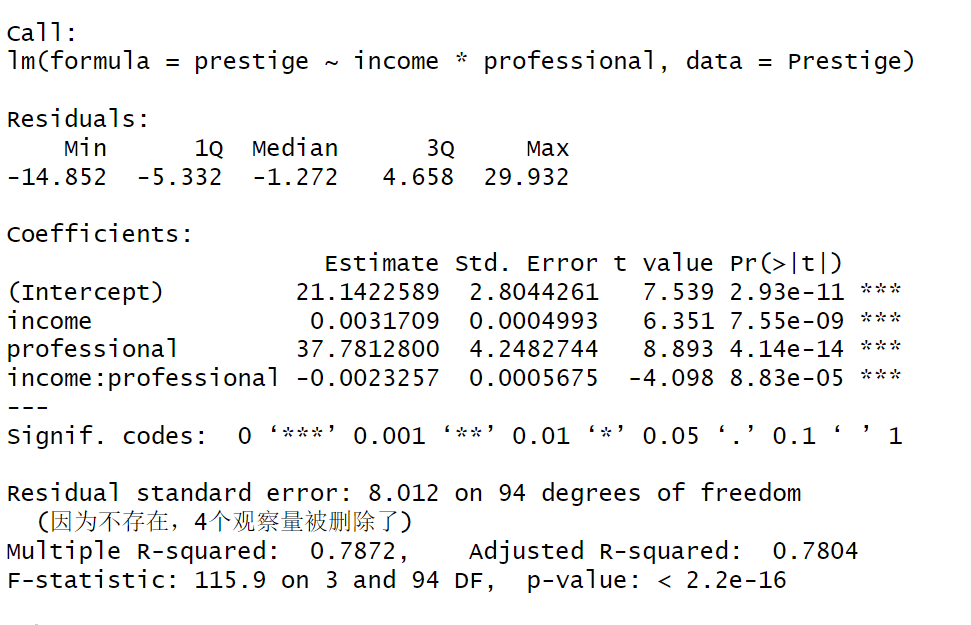
\includegraphics[width=0.8\textwidth]{Q1_b1.png}\\
	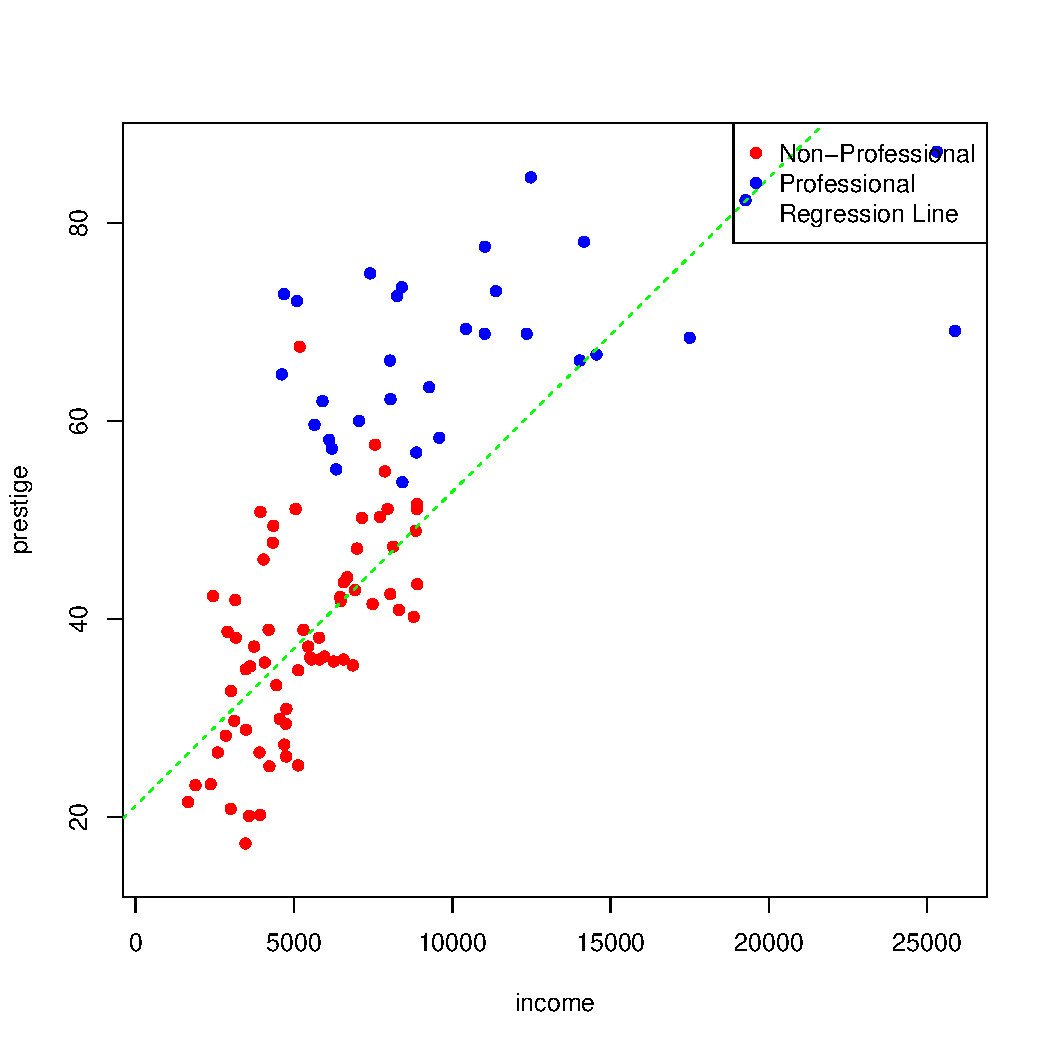
\includegraphics[width=.85\textwidth]{Q1_b.pdf} 
	
	\item [(c)]
	Write the prediction equation based on the result.
	
	\vspace{.25cm}
	\lstinputlisting[language=R, firstline=64, lastline=75]{PS4_zhuo_zhang.R} 
	\textbf{Result}:\\
	prediction equation:prestige = 21.14 + 0 * income + 37.78 * professional + 0 * income * professional\\
	
	
	\item [(d)]
	Interpret the coefficient for \texttt{income}.
	\vspace{.25cm}\\
	\textbf{Result}:\\
	The coefficient of the ``income'' variable is 0, indicating that ``income'' has no effect on the predicted prestige score in the model. The coefficient is 0 means that there is no linear relationship between ``income'' and ``prestige''.
	\item [(e)]
	Interpret the coefficient for \texttt{professional}.
	\vspace{.25cm}\\
	\textbf{Result}:\\
		The coefficient of the 'professional' variable is 37.78, indicating that when the 'professional' variable changes from 0 to 1 (indicating a professional profession compared to non professional), the predicted prestige score is expected to increase by 37.78 units. This coefficient indicates a positive linear relationship between professional occupation and prestige scores.
	
	\item [(f)]
	What is the effect of a \$1,000 increase in income on prestige score for professional occupations? In other words, we are interested in the marginal effect of income when the variable \texttt{professional} takes the value of $1$. Calculate the change in $\hat{y}$ associated with a \$1,000 increase in income based on your answer for (c).
	\vspace{.25cm}\\
	\textbf{Result}:\\
	prediction equation:prestige = 21.14 + 0 * income + 37.78 * professional + 0 * income * professional\\
	Since the coefficient of the ``income'' variable is 0, it indicates that ``income'' has no effect on the predicted prestige score in the model, so an increase of \$1000 in income has no effect on the reputation of professionals.
	
	
	\item [(g)]
	What is the effect of changing one's occupations from non-professional to professional when her income is \$6,000? We are interested in the marginal effect of professional jobs when the variable \texttt{income} takes the value of $6,000$. Calculate the change in $\hat{y}$ based on your answer for (c).
	\vspace{.25cm}\\
	\textbf{Result}:\\
	prediction equation:prestige = 21.14 + 0 * income + 37.78 * professional + 0 * income * professional\\
	When professional = 1 and income = 6,000:\\
	prestige = 21.14 + 0 * 6000 + 37.78 * 1 + 0 * 6000 * 1\\
	prestige = 58.92\\
	When professional =0 and income = 6,000:\\
	prestige = 21.14 + 0 * 6000 + 37.78 * 0 + 0 * 6000 * 0\\
	prestige = 21.14\\
	58.92 - 21.14 = 37.78\\
	The change in the predicted prestige score associated with changing one's occupation from non-professional to professional when income is $6,000$ is 37.78.\\
	
	
\end{enumerate}

\newpage

\section*{Question 2: Political Science}
\vspace{.25cm}
\noindent 	Researchers are interested in learning the effect of all of those yard signs on voting preferences.\footnote{Donald P. Green, Jonathan	S. Krasno, Alexander Coppock, Benjamin D. Farrer,	Brandon Lenoir, Joshua N. Zingher. 2016. ``The effects of lawn signs on vote outcomes: Results from four randomized field experiments.'' Electoral Studies 41: 143-150. } Working with a campaign in Fairfax County, Virginia, 131 precincts were randomly divided into a treatment and control group. In 30 precincts, signs were posted around the precinct that read, ``For Sale: Terry McAuliffe. Don't Sellout Virgina on November 5.'' \\

Below is the result of a regression with two variables and a constant.  The dependent variable is the proportion of the vote that went to McAuliff's opponent Ken Cuccinelli. The first variable indicates whether a precinct was randomly assigned to have the sign against McAuliffe posted. The second variable indicates
a precinct that was adjacent to a precinct in the treatment group (since people in those precincts might be exposed to the signs).  \\

\vspace{.5cm}
\begin{table}[!htbp]
	\centering 
	\textbf{Impact of lawn signs on vote share}\\
	\begin{tabular}{@{\extracolsep{5pt}}lccc} 
		\\[-1.8ex] 
		\hline \\[-1.8ex]
		Precinct assigned lawn signs  (n=30)  & 0.042\\
		& (0.016) \\
		Precinct adjacent to lawn signs (n=76) & 0.042 \\
		&  (0.013) \\
		Constant  & 0.302\\
		& (0.011)
		\\
		\hline \\
	\end{tabular}\\
	\footnotesize{\textit{Notes:} $R^2$=0.094, N=131}
\end{table}

\vspace{.5cm}
\begin{enumerate}
	\item [(a)] Use the results from a linear regression to determine whether having these yard signs in a precinct affects vote share (e.g., conduct a hypothesis test with $\alpha = .05$).
	\vspace{.25cm}\\
	\textbf{Result}:\\
	Precinct assigned lawn signs:\\
	Coefficient = 0.042\\
	Standard error = 0.016\\
	To determine whether having these yard signs in a precinct affects vote share:\\
	Hypothesis Test:\\
	Coefficient for "Precinct assigned lawn signs"\\
	H0: Coefficient  = 0 (no effect)\\
	H1: Coefficient  $\neq$ 0(have effect)\\
	t = $\frac{Coefficient}{Standard Error}$ = $\frac{0.042}{0.016}$= ${2.625}$ \\
	The critical value for a two-tailed test with  $\alpha = .05$ = 0.05 is approximately 1.96.\\
	For 2.625 $>$ 1.96 ,\\
	I can reject the null hypothesis and conclude that the variable "Precinct assigned lawn signs" has a significant effect on vote share.\\
	
			
	\item [(b)]  Use the results to determine whether being
	next to precincts with these yard signs affects vote
	share (e.g., conduct a hypothesis test with $\alpha = .05$).
	\vspace{.25cm}\\
	\textbf{Result}:\\
	Precinct adjacent to lawn signs:\\
	Coefficient = 0.042\\
	Standard error = 0.013\\
	To determine whether being next to precincts with these yard signs affects vote share:\\
	Hypothesis Test:\\
	Coefficient for "Precinct adjacent to lawn signs"\\
	H0: Coefficient  = 0 (no effect)\\
	H1: Coefficient  $\neq$ 0(have effect)\\
	t = $\frac{Coefficient}{Standard Error}$ = $\frac{0.042}{0.013}$= ${3.231}$ \\
	The critical value for a two-tailed test with  $\alpha = .05$ = 0.05 is approximately 1.96.\\
	For 3.231 $>$ 1.96 ,\\
	I can reject the null hypothesis and conclude that the variable "Precinct adjacent to lawn signs" has a significant effect on vote share.\\
	
	\item [(c)] Interpret the coefficient for the constant term substantively.
	\vspace{.25cm}\\
	\textbf{Result}:\\
	The coefficient for the constant term is 0.302.\\
	It represents the expected vote share when all predictor variables (Precinct assigned lawn signs and precinct adjacent to lawn signs) are zero.\\
	It is the expected vote share when there are no yard signs and no adjacency to yard signs.\\
	
	
	
	\item [(d)] Evaluate the model fit for this regression.  What does this	tell us about the importance of yard signs versus other factors that are not modeled?
	\vspace{.25cm}\\
	\textbf{Result}:\\
	$R^2$=0.094,\\
	The correlation coefficient $R^2$ is a statistical indicator of the degree of correlation between two variables, which can reflect the strength of the correlation between two variables in the linear relationship. the larger the $R^2$, the stronger the relationship between the two variables, the more significant the linear relationship between the variables; on the contrary, the smaller the $R^2$, the weaker the relationship between the two variables, the linear relationship between the variables is not significant.\\
	
	$R^2$=0.094, the $R^2$ is low, it suggests that the model does not explain a large proportion of the variability in the dependent variable.\\
	
	In summary, as included in the model, explain only a small portion of the variability in the vote share. Other unmodeled factors are likely influencing voting preferences to a greater extent. We need to consider additional other variables, as well as refine the model in order to find the important factors that I influence the outcome of the election.\\
\end{enumerate}  


\end{document}
